%----------------------------------------------------------------------------
%\chapter{\Kubernetes}
%\label{sec:Kubernetes}
%----------------------------------------------------------------------------
\chapter{Kubernetes}
\label{sec:Kubernetes}
A félévben végzett munka jelentős mértékben támaszkodik a Kubernetes (K8s) rendszerre, így annak ismertetése szükségszerű. 

%----------------------------------------------------------------------------
\section{Motivációja}
%----------------------------------------------------------------------------
Ahogy egyre többen kezdték megismerni és használni a konténerizációs technikákat, mint például a Docker, úgy egyre tolódott át az üzemeltetési oldal is ilyen irányba. Ezek után nem  az jelentette a kihívást, hogy az egyes alkalmazásokat egy dedikált virtuális gépen kellett beüzemelni és elindítani. Az új igények szerint az alkalmazásunk egyes részeit egymástól függetlenül kellett konténerekben futtatni. Ezáltal sokkal több kisebb részegységre kellett figyelni, ami jelentősen több feladattal jár, mint a korábbi gépek kezelése. 

Ezzel a problémával találkozott a Google is és kezdődött egy platform fejlesztése, ami képes a fenti feladatok megoldására. Eleinte ez a \textit{Borg}\citep{Borg} nevet viselte. Ezt 2014-ben a Google nyílt forráskódúvá tette immáron Kubernetes néven. A projektet a \textit{Cloud Native Computing Foundation (CNCF)} vette gondozásába. Innentől kezdve bárki szabadon elérheti és bele is fejleszthet. Az elmúlt 6 év alatt hatalmas fejlődésen ment keresztül és már a $22$.-ik kiadásánál tart.

%----------------------------------------------------------------------------
\section{Felépítése}
%----------------------------------------------------------------------------
erőforrások: CPU és memoria

\subsection{Objektumok}
%----------------------------------------------------------------------------
A Kubernetes egyik erőssége, hogy az átlagos felhasználás esetében nem kell törődni a rendszer felépítésével, hiszen nekünk csak deklaratív módon meg kell létrehozni és kezelni bizonyos erőforrásokat, objektumokat.
  
\paragraph{Pod}
A Kubernetesben megjelenő legkisebb egység. Általában egy konténert futtat, de lehetőségünk van több konténer futtatására is. Általánosságban elmondható, hogy rendszeresen létrejönnek és rendszeresen törölve is lesznek ezek az objektumok, tehát nem tartós életűek. Ez az egész rendszernek tud adni egy 

\paragraph{ReplicaSet} 
Az ő feladata, hogy bizonyos \textit{Podból} megfelelő számú egység fusson. Ennek értelmében, ha az egyik \textit{Pod} meghibásodik és megáll, akkor helyette egy újat fog létrehozni. Ezzáltal biztosított, hogy mindig a megfelelő számú egység fogja fogadni a beérkező kéréseket és nem kell munálisan monitorozni a státuszukat.

\paragraph{Deployment}
Mivel \textit{Podok} 

\paragraph{Service}
asd

%----------------------------------------------------------------------------
\section{Skálázás}
%----------------------------------------------------------------------------
A felhős infrasturktúra egyik legcsábítóbb előnye, hogy az alkalmazásunk képes adaptálódni a külvilág felől érkező kérésekhez. Ez azt jelenti, hogy ha több felhasználót kell egyszerre kiszolgálni, akkor a rendszer autómatikusan növeli a kiszolgálásra fordított erőforrások mennyiségét. Ezzel a megoldással elérhetjük, hogy a végfelhasználó ne vegyen észre minőségbeli csökkenést és a kevésbé intenzív időkben pedig nem foglalunk feleslegesen erőforrást, ami az üzemeltetőnek is jól belátható anyagi érdeke.
 
Alapvetően két különböző skálázási módszert lehet elkülöníteni. Az egyik a vertikális, míg a másik a horizontális skálázás. Ezekről a későbbiekben bővebben lesz szó. 

\subsection{Horizontális skálázás}
%----------------------------------------------------------------------------
A két skálázási mód közötti különbséget mutatja a \refstruc{fig:scaling}. Jobb oldalon látható megoldás az úgynevezett horizontális skálázás (másnevén: scaling out). Ebben az esetben arról van szó, hogy a megnövekedett igények kiszolgálásához több azonos egységet hozunk létre. Az összes egység azonos erőforrás felhasználásra

Előnye: könnyű kezelni, elepértelmezetten támogatott, 
Hátránya: amdal törvénye

% amdal törvénye

\subsection{Vertikális skálázás}
%----------------------------------------------------------------------------
Tud ilyet is, alapból nem támogatott.

Hátrány: nehezebb implementáció, nem növelhető végtelenségig (pl: ha az alkalmazás nem támogatja a többszálas futtatást.)
előny: nincs sinkronizációs overhead


% Skálázás módjai ábra -------------------------------------------------------
\begin{figure}[!ht]
\centering
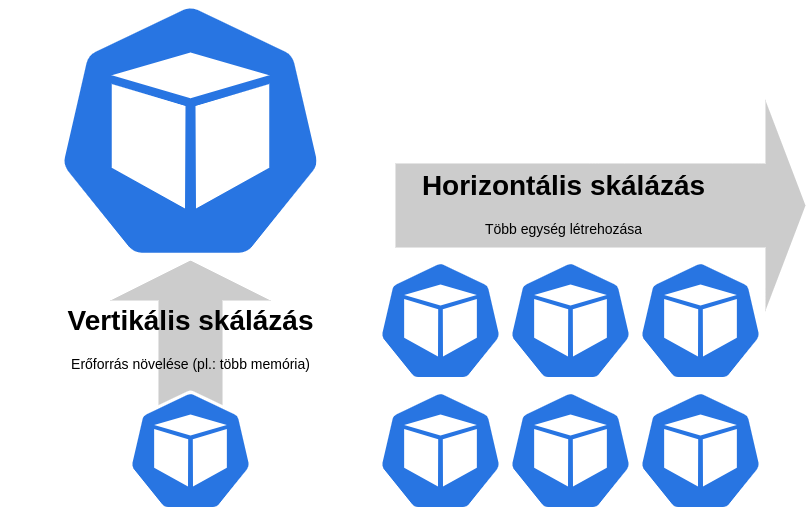
\includegraphics[width=150mm, keepaspectratio]{figures/scaling_types.png}
\caption{Vertikális és horizontális skálázás}
\label{fig:scaling}
\end{figure}
